% The prose of results/e89eb7ad-umbilicus-estimator, first published on 2026-09-17 as lines 74 to
% 1112 of paper/00001/paper/papers/umbilicus-score-patch.tex of the laboratory and moved here on
% 2026-09-23 with the four figure paths renamed to figures/<stem>.
% Style pass of 2026-09-28 (director 18:27:58Z, the owner's word): no bold in running text, narrative
% paragraphs, provenance pointers in footnotes. Every macro, figure and table is as it was.
% Lean pass of 2026-09-30 (brief-lean-pass-2026-09-30, the owner's word): one introduction in place of
% the opening, the plain words section and its glossary; the dated addendum removed, with the state of
% pull request 1823 in one sentence of the introduction and the author's closed pull requests no longer
% named; the post hoc material tightened; limits, open questions and conclusion rewritten from the text
% already here. No macro changes value and no figure or table changes.

\begin{abstract}
The umbilicus estimator of Volume Cartographer scores a candidate centre with a weighted sum of
squared cosines divided by the sum of the weights, a weighted mean. We show
that the limit of that mean far from the section is the largest eigenvalue of the normals'
covariance. Where this limit exceeds the score on the axis, the hill climb walks out of
the volume. The published estimate leaves the grid on
\RevFarRunaways\ of \RevFarSlicesTotal\ slices, and \RevFarTruePos\ of those meet the condition.
Without the division the score is a weighted sum, with a maximum at finite distance. The
change is one line, now merged into the challenge's code. On a run of \RevRunScrolls\
scrolls it keeps \RevGenInsideFixed\ of \RevGenSlices\ slices inside the grid, against
\RevGenInsideAsIs\ as published. Only \RevGenCritPassed\ of its four registered criteria pass, so the
run does not show that the change generalises. Against the centroid of the sheet mask, by a margin fixed
in advance, the sum wins on \RevKConfirmBeats\ of \UmbConfirmScrolls\ third party references,
out of sample. It costs a bias towards the denser side. The error of the hand references
remains unmeasured, and we do not claim that the weighted sum is the right objective.
\end{abstract}

\begin{IEEEkeywords}
Herculaneum papyri, virtual unwrapping, umbilicus, objective functions, software defects,
pre-registration.
\end{IEEEkeywords}

\begin{figure*}[t]
\centering
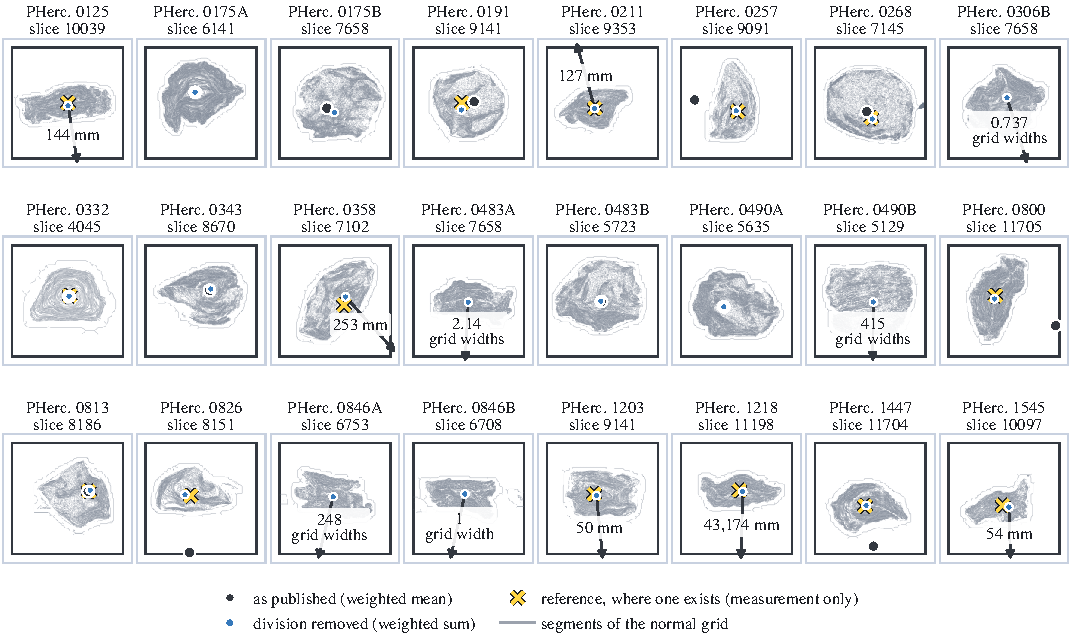
\includegraphics[width=\textwidth]{figures/umbilicus-gallery-24}
\caption{\RevGalleryCaption}
\label{fig:gallery}
\end{figure*}

\section{Introduction}
\label{sec:line}

\IEEEPARstart{T}{he} organisers of the Vesuvius Challenge name as their next goal, in their list
of open problems for 2026, ``making all of this reliable, on any scroll, without someone catching
every failure''~\cite{openproblems2026}. The scrolls of Herculaneum were carbonised by the eruption
of Vesuvius and cannot be opened by hand. They are scanned in three dimensions, and software has to
find the rolled sheet inside the scan. Spiral fitting~\cite{henderson} reconstructs that sheet by
fitting the whole spiral at once, and it has one input that cannot be omitted: the umbilicus. That
is the line through the centre of the roll, with one point per slice, a slice being one horizontal
section of the scan at one height. The umbilicus is drawn by hand~\cite{umbmaker}, the challenge
publishes one for a small minority of its scrolls, and on the rest it has to be estimated before
anything else can be attempted. A centre found without a person to check it removes one manual
step, on every scroll, between a scan and a sheet that someone can read.

\texttt{volume-cartographer}~\cite{villa}, the toolchain of the challenge's \texttt{villa}
repository, contains an estimator for exactly this. It is the function \fn, defined at
\cppline{15}, whose header comment calls it ``a RANSAC-based approach to find a common umbilicus
point''. It reads the normal grid, the published directions of the sheets of a scroll,
perpendicular to the papyrus. It samples line segments from the grid and scores a candidate centre
by how well the directions from the candidate to the segments line up with their normals. It then
picks the best of a thousand random candidates and refines it with a hill climb, a search that
moves the candidate step by step towards a higher score. At the commit we measured, nothing in the
repository calls the function but its own tests. Every
line number in this paper refers to commit \texttt{\RevVillaShort}. At \texttt{\RevUpstreamTip},
the tip of the default branch on \RevUpstreamDate, the line at issue was still line
\RevUpstreamDefectLine. That tip is \RevUpstreamAhead\ commits later, and \RevUpstreamTouching\ of
those commits touch the source file or its header.

We show that the score the function refines is a weighted mean whose limit far from the section
can exceed its value on the axis. The hill climb then walks out of the scan
(Section~\ref{sec:defect}). Removing the division turns the mean into a weighted sum, which has a
maximum at finite distance. We measure the compiled function with and without the division
against the fifteen scrolls that carry a hand drawn umbilicus, under verdicts written before the
run (Sections~\ref{sec:fifteen} and~\ref{sec:baselines}). We also run it on the \RevRunInCompetition\ scrolls of the
competition set and \RevRunNotInCompetition, under four criteria registered before that run
(Section~\ref{sec:twentyfour}). We then measure what the change costs (Section~\ref{sec:density})
and whether the search shared the fault (Section~\ref{sec:ablation}). The patch
(Section~\ref{sec:patch}) is that line, a seed argument that makes a run repeatable, and a
regression test on synthetic sections whose centre is known. Pull request \UpPatchPR~\cite{villapr},
which carries it, was merged into the main branch of \texttt{villa} on \NowPatchMergedLong\ at
\NowPatchMergedTime.\footnote{As the GitHub API gave it when read again on \NowReadLong\ at
\NowReadTime.}

The function, the normal grids and the reference umbilici are not ours. The first two are the
challenge's, and the references are the challenge's and a third party's (Section~\ref{sec:fifteen}).
Ours are the analysis, the measurements, the patch and the tools that write every number. A reader
can check each number without taking it on trust: the appendix names, for each section, table and
figure, the file its numbers are read from and the tool that writes that file. The rules the
verdicts were judged by were written and dated before the measurements~\cite{nosek2018}. They
are in \texttt{src/prereg/}, and those of the run on the \RevRunScrolls\ scrolls and of the
twenty seeds are in \texttt{src/inputs/}.

\section{The defect}
\label{sec:defect}
This section shows why dividing by the sum of the weights gives the score an attractor far from
the scroll, and then tests that account on every slice that has a reference.

\begin{figure}[t]
\centering
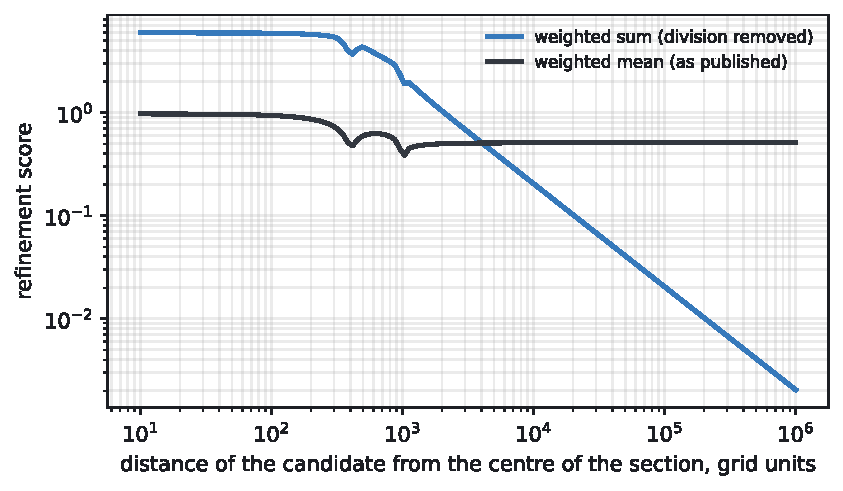
\includegraphics[width=\columnwidth]{figures/normalgrid-mechanism}
\caption{Refinement score of \cppline{98-117} on a synthetic section, one turn of a spiral of
4000 sampled points, against the distance of the candidate from the centre of the section.
Weighted sum and weighted mean, same section, same samples. Recomputed by
\texttt{tools/synthetic\_density.py} on this section and on a concentric circle
(\texttt{evidence/mechanism-curve.csv}): a million units away the sum retains
\RevMechSpiralSumFar\ of its maximum and the mean \RevMechSpiralMeanFar; on the circle,
\RevMechCircleSumFar\ and \RevMechCircleMeanFar.}
\label{fig:mechanism}
\end{figure}

The refinement score runs over sampled segment midpoints, weights each by the inverse of its
distance from the candidate and adds up the squared cosine between the segment normal and the
direction to the segment. The last line of it divides (\cppline{112-116}):

\begin{center}
\begin{minipage}{0.93\columnwidth}
\footnotesize
\begin{verbatim}
float weight = 1.0f / std::max(100.0f, dist);
score += (cos_angle * cos_angle) * weight;
wsum  += weight;
...
return score/wsum;
\end{verbatim}
\end{minipage}
\end{center}

Without that division the quantity is a weighted sum. Let $D$ be the distance of the candidate
from the section and $\mathbf{u}$ the unit vector from the candidate towards it. Every weight
tends to $1/D$, so the sum tends to zero: a positive continuous function that vanishes at infinity
attains a maximum at finite distance, by construction. With the division it is a weighted mean.
Numerator and denominator vanish together, and every direction from the candidate to a segment
tends to $\mathbf{u}$. The limit far from the section, which we call the far field, is then the
plain mean of the squared cosines over the $N$ sampled normals $\mathbf{n}_i$,
\begin{equation}
\lim_{D\to\infty}\frac{\sum_i w_i\cos^2\theta_i}{\sum_i w_i}
  = \frac{1}{N}\sum_{i=1}^{N}(\mathbf{n}_i\cdot\mathbf{u})^2
  = \mathbf{u}^{\mathsf{T}}C\,\mathbf{u},
\label{eq:farfield}
\end{equation}
with $C=\frac{1}{N}\sum_i\mathbf{n}_i\mathbf{n}_i^{\mathsf{T}}$. Every normal contributes equally
to that limit, however far it is, because a mean does not know how many normals are contributing
or where they are. On a complete circle of radial normals the limit is $1/2$ for every
$\mathbf{u}$. On a partial section whose normals are coherent it rises towards 1 along the mean
normal. It can exceed the score at the true centre once the normals there are noisy, so the mean
stays high far away while the sum collapses (Fig.~\ref{fig:mechanism}).

The maximum of that limit over $\mathbf{u}$ is the largest eigenvalue of $C$. That turns the
observation of Fig.~\ref{fig:field} into a criterion computable from the normals alone: the defect
strikes partial predictions with coherent normals and spares complete sections. The criterion can
be measured on the samples the estimator itself draws, \RevFarSamples\ of
them.\footnote{\texttt{tools/far\_field\_eigenvalue.py}, which writes
\texttt{evidence/far-field-eigenvalue.csv}.} On the \RevFarSliceScroll\ slice of
Fig.~\ref{fig:field} the largest eigenvalue is \RevFarSliceLambda, while the weighted mean at the
published control point is \RevFarSliceCentre. The far field is therefore \RevFarSliceRatio\ times
the score at the centre, and the climb has somewhere better to go. A synthetic full circle gives
\RevFarCircleLambda\ against \RevFarCircleCentre\ at the centre. A half circle of radial normals
still gives \RevFarHalfLambda, because normals spanning half a turn cover both directions of the
plane as evenly as normals spanning the whole of it. That is why the maximum of the mean sits at
the true centre on the half circle of Table~\ref{tab:density}, \RevDensHalfMeanFieldErr\ units away
against \RevDensHalfSumFieldErr\ for the sum. The one section of that table where it does not is
the ellipse, where it sits \RevDensEllipseMeanFieldErr\ units away, against \RevDensEllipseSumFieldErr\
for the sum.
It is also why the one complete concentric section of the primary block, PHerc0332, gives the same
median with and without the division, \RevKZeroThreeThreeTwoAsIs\ against
\RevKZeroThreeThreeTwoMedian~mm in Table~\ref{tab:primary}. What changes there is the count of
runs outside the grid: \RevKZeroThreeThreeTwoOutsideAsIs\ of \RevKInsideOf\ as published, against
\RevKZeroThreeThreeTwoOutsideFixed\ with the division removed.

\begin{figure}[t]
\centering
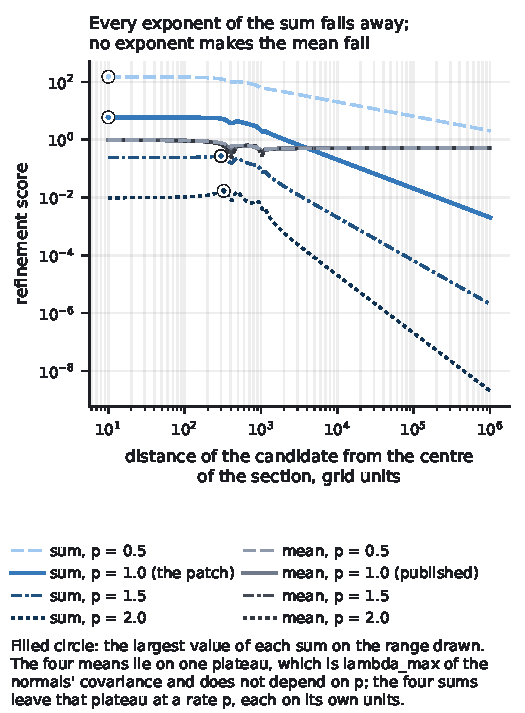
\includegraphics[width=\columnwidth]{figures/exponent-mechanism}
\caption{The same score against the same distance as Fig.~\ref{fig:mechanism}, with the exponent of
the weight set to \RevExpList. The four weighted means end on one plateau, the largest eigenvalue
of $C$, which does not depend on the exponent. The four weighted sums leave it downwards with slope
$p$. Drawn by \texttt{tools/figure\_exponent.py} from
\texttt{evidence/exponent-ablation-mechanism-curve.csv}; the rate at which each curve approaches
or leaves the plateau is measured in \texttt{evidence/exponent-ablation-cancellation-rate.csv}.}
\label{fig:exponent}
\end{figure}

A faster falling weight does not rescue the mean, because a pure power cancels. With weights
$1/d_i^{\,p}$ the factor $D^{-p}$ stands in the numerator and in the denominator alike and leaves
equation~(\ref{eq:farfield}) as it is. The sum keeps the factor and vanishes as $D^{-p}$ for every
$p>0$. A larger exponent moves the distance at which the plateau becomes visible; it does not lower
the plateau (Fig.~\ref{fig:exponent}), and Section~\ref{sec:exponent} measures the exponent on the
fifteen scrolls.

The two objectives therefore fail on orthogonal properties. The mean fails when the normals of a
section are coherent, which is what the eigenvalue measures. It is exact when they cover the
plane however one-sided the section is, as the half circle shows. The sum fails when the density
of the segments is asymmetric, which is what Section~\ref{sec:density} measures, and coherence
does not trouble it. A real prediction is usually both at once, partial and one-sided, so neither
objective is right in general, and our choice is made for the sections this toolchain actually
processes.

\begin{table}[t]
\caption{Equation~(\ref{eq:farfield}) with the scroll as the unit, the \RevFarScrollSlicesEach\
slices of each of the \RevFarScrollUnit\ scrolls with a manual reference. Flagged: slices where the
far field bound exceeds the weighted mean at the reference control point. Left: slices whose
estimate as published leaves the grid, by the rule of Table~\ref{tab:farfield}. Missed: leaving
runs the condition did not flag. Generated from \texttt{evidence/far-field-per-scroll.csv}.}
\label{tab:farfieldscrolls}
\centering
\footnotesize
\begin{tabular}{@{}lrrrr@{}}
\toprule
scroll & flagged & left & flagged and left & missed \\
\midrule
\inputrows{rev1-far-field-scrolls}
\bottomrule
\end{tabular}
\end{table}

\begin{table}[t]
\caption{Equation~(\ref{eq:farfield}) against the runs, on the \RevFarSlicesTotal\ slices of the
\RevFarScrolls\ scrolls with a manual reference. Rows: whether the far field bound exceeds the
weighted mean at the reference control point of that slice. Columns: whether the estimate as
published leaves the grid, by the rule fixed before the run, \RevFarSliceSeedRule\ landing
outside. Generated from \texttt{evidence/far-field-prediction.csv}.}
\label{tab:farfield}
\centering
\footnotesize
\begin{tabular}{@{}lrr@{}}
\toprule
 & leaves the grid & stays inside \\
\midrule
$\lambda_{\max} >$ mean at the reference & \RevFarTruePos & \RevFarFalsePos \\
$\lambda_{\max} \leq$ mean at the reference & \RevFarFalseNeg & \RevFarTrueNeg \\
\bottomrule
\end{tabular}
\end{table}

Equation~(\ref{eq:farfield}) speaks about every slice, so we put it to every slice that has a
reference, the hand drawn umbilicus of Section~\ref{sec:fifteen}. An estimate leaves the grid when
it ends outside the bounds of the scan. That is \RevFarSlicesTotal\ slices on the \RevFarScrolls\
scrolls with a manual reference, the \RevFifteenSlices\ slices of each scroll that
Section~\ref{sec:fifteen} measures, run with the same \RevKSeeds\ seeds per slice. For each slice
we computed two things on the samples the table's own seed draws: the largest eigenvalue of $C$,
and the weighted mean at that slice's reference control point.\footnote{By
\texttt{tools/far\_field\_eigenvalue.py}.} The reference serves only to evaluate the score at a
point known to lie on the axis, which is measuring and not choosing.

Table~\ref{tab:farfield} gives the answer. The bound exceeds the score on the axis on
\RevFarPredictedYes\ slices. The published estimate leaves the grid on \RevFarRunaways, and
\RevFarTruePos\ of those satisfy the condition. Of the \RevFarPredictedNo\ slices where the bound
stays below the axis, \RevFarFalseNeg\ walk out. The condition is therefore \RevFarNecessity. Its
sensitivity is \RevFarSensitivity\ and its specificity \RevFarSpecificity. The \RevFarFalsePos\
slices that satisfy it and stay inside are those where the climb does not reach the border from its
random start, which the criterion does not claim to predict.

The outcomes here are those of the shipped walk, from the same \RevKSeeds\ seeds per slice as the
tables. The eigenvalues come from the grids and are the same under either instrument. Against the
transcription's outcomes on the same slices, \RevFarSidesChanged\ slices change side under the
majority rule. They are \RevFarSidesChangedSlices. \RevFarMissSentence

Those \RevFarSlicesTotal\ slices are not independent observations. They are
\RevFarScrollSlicesEach\ from each of \RevFarScrollUnit\ scrolls, and slices of one scroll share a
geometry, a surface prediction and a scanner, so a test that pools them would answer a question
nobody asked. With the scroll as the unit no pooling is needed. On \RevFarScrollsZeroMisses\ of the
\RevFarScrollUnit\ scrolls, not one run that left the grid escaped the condition. Runs left the grid
on \RevFarScrollsWithLeaving\ scrolls, and on \RevFarScrollsAllFlagged\ of them every leaving run was
flagged (Table~\ref{tab:farfieldscrolls}). The remaining scroll, \RevFarScrollNoLeaving, has no run
to flag. To test the pairing, we shuffled the predictor among the slices of one scroll,
independently in each scroll, which holds every scroll's own two counts fixed and breaks only the
pairing between them. The statistic is a sum over scrolls of independent hypergeometric counts, so
its tail under that null is exact by convolution: $p$~$=$~\RevFarPermExactP. A simulation agrees.
Of \RevFarPermRounds\ shuffles, \RevFarPermHits\ reached the observed count, so
$p$~$<$~\RevFarPermP.

The hill climb at \cppline{119-142} is therefore not searching for a maximum that is hard to
find. On most real sections it is searching for one that is not there, and it keeps stepping
outwards because every step improves the mean a little. Nothing stops the walk: \cppline{128} adds
the step to the current best with no clamp to the grid. The answer can leave the volume by an
arbitrary distance, and the routine still returns it as an estimate.

\begin{figure*}[t]
\centering
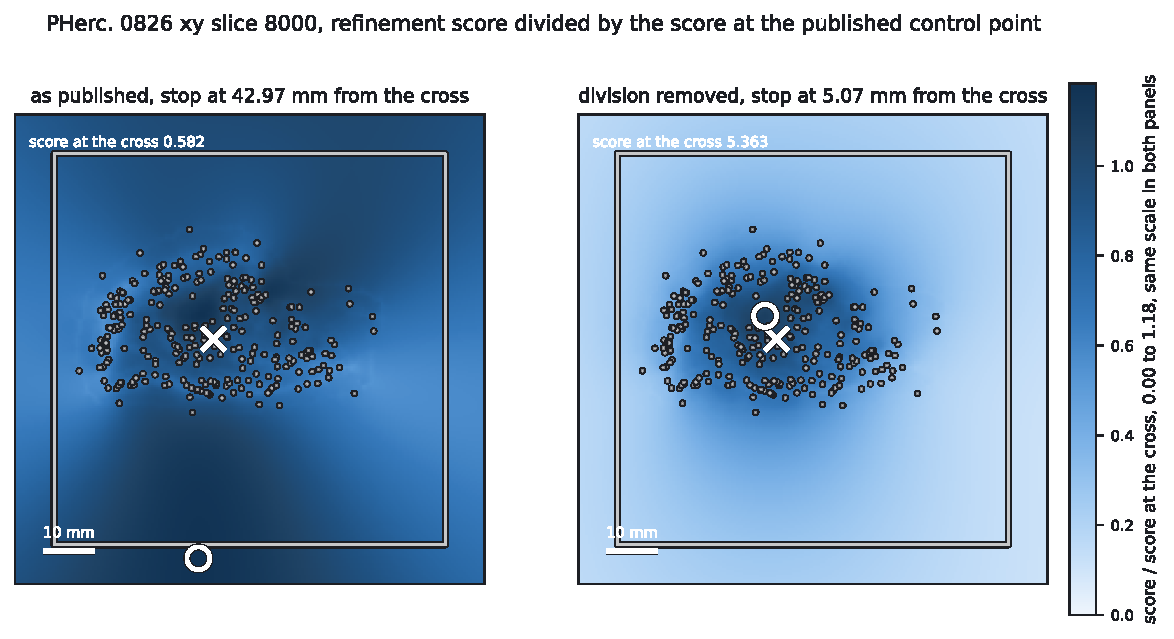
\includegraphics[width=\textwidth]{figures/normalgrid-score-field}
\caption{Refinement score over PHerc.\ 0826, xy slice 8000, divided in each panel by the score at
the published control point, so that both panels carry the same dimensionless scale. Left: as
published, the weighted mean. Right: the weighted sum. Cross: the published control point.
Circle: where the hill climb of \cppline{119-142} stops. Rectangle: the bounds of the grid. Dots: one sampled segment midpoint in 80. Bar: 10 mm at 9.362 um per voxel. Drawn by
\texttt{inputs/figure\_umbilicus.py} from that slice of the published normal grids and from the
reference umbilicus of PHerc.\ 0826.}
\label{fig:field}
\end{figure*}

Fig.~\ref{fig:field} is one real slice scored both ways, on one scale. A weighted mean and a
weighted sum do not have the same units, so both panels are divided by the score at the published
control point, which is the same physical place in both. As published, the field rises towards one
edge of the grid and is as high far from the sheets as it is at the control point. Its maximum
sits on that edge and not on the sheets. The climb stops \UmbFieldStopAsIs~mm from the control
point, outside the grid. With the division removed the field collapses away from the sheets, the
maximum sits inside the cloud of sheet segments, and the climb stops \UmbFieldStopFixed~mm from
the control point. In both cases the hill climb finds what its objective tells it to find.

The other score the function computes does not repair this. The candidate selection of lines 78
to 88, which picks the seed for the refinement, is an unweighted sum of the same squared cosines.
It carries no distance weight at all, so nothing in it localises a maximum, and on the slices where
the published objective peaks at the border that one does too. Dividing by the number of samples
would change nothing, while dividing by the sum of the weights moves the maximum, because that sum
depends on where the candidate is.

What the argument guarantees is narrower than what the measurement finds. A weighted sum whose
weights fall as $1/D$ has a maximum at finite distance for every section, of any shape, at any
resolution. But that maximum is interior to the plane and not to the grid, and the argument bounds
the objective and not the number of sweeps the search takes to reach it. That every estimate lies
inside the volume, and that every walk stopped by itself, are empirical results:
\RevGenInsideFixed\ of \RevGenSlices\ in Section~\ref{sec:twentyfour}. Where the maximum sits is not
guaranteed either, and Section~\ref{sec:density} measures it.

\section{Against fifteen manual references}
\label{sec:fifteen}
This section measures the compiled function against the fifteen scrolls that carry a hand drawn
umbilicus, and applies to it the verdicts that were written before the run.

\begin{table*}[t]
\caption{Primary block: the \UmbPrimaryScrolls\ umbilici published by the Vesuvius Challenge, one
of them annotated by David Josey. Every rule is scored on the same \RevFifteenSlices\ slices of the
same scroll; the estimate is a polyline through those slices and the distance is taken at each of
the scroll's control points, in millimetres of the scan the reference is annotated on, so the row
is a median over \RevFifteenCpMin\ to \RevFifteenCpMax\ control points, not over slices. Bold is
the estimator with the weighted sum, estimated with \RevKSeeds\ seeds per slice: the median over
the \RevKSeeds\ per-seed medians, its 95 \% percentile bootstrap interval in brackets
(\RevKResamples\ resamples, one seed drawn per slice and the control points resampled, generator
seed \RevKBootSeed). The margin is centroid minus estimator; $^{\circ}$ marks a margin whose
interval includes zero, and $^{\dagger}$ a margin smaller than \UmbReferenceSpread~mm. That
distance separates the hand annotation of PHerc.\ 1218 from a per slice centroid of the papyrus
mask~\cite{dopico}, not one hand from another, and it sits \SecRefPublishedVsCentroidMm~mm from
that scroll's own centroid column in Table~\ref{tab:confirm}, so the dagger reads as a margin
smaller than the baseline's own distance from the reference, which is close to circular. It is
kept because the pre-registration fixed the marking before any of these numbers were seen;
Section~\ref{sec:notdone} gives the size of the overlap. It is a reading aid and not a
criterion. The last column counts estimates outside the grid over all \RevKInsideOf\ runs, as
published and with the division removed. Generated from \texttt{evidence/cpp-k20.csv}.}
\label{tab:primary}
\centering
\footnotesize
\setlength{\tabcolsep}{3.5pt}
\begin{tabular}{@{}lrrlrrlc@{}}
\toprule
scroll & points & published & \textbf{with the sum} [95 \%] & centroid & axis & margin [95 \%] & outside \\
\midrule
\inputrows{rev1-k20-primary}
\bottomrule
\end{tabular}
\end{table*}

\begin{table*}[t]
\caption{Confirmation block: \UmbConfirmScrolls\ manual references of a third party,
\texttt{herculaneum-umbilici}~\cite{drobkov}, MIT, clicked on level 3 images at scale 8, one slice
every about 480 in z, by someone who was not annotating for this purpose. A weaker reference by
construction, kept in a block of its own and never pooled with Table~\ref{tab:primary}. Columns
and marks as in Table~\ref{tab:primary}. Generated from \texttt{evidence/cpp-k20.csv}.}
\label{tab:confirm}
\centering
\footnotesize
\setlength{\tabcolsep}{3.5pt}
\begin{tabular}{@{}lrrlrrlc@{}}
\toprule
scroll & points & published & \textbf{with the sum} [95 \%] & centroid & axis & margin [95 \%] & outside \\
\midrule
\inputrows{rev1-k20-confirm}
\bottomrule
\end{tabular}
\end{table*}

\begin{table*}[t]
\caption{Two more rules, scored after the fact. The plateau point nearest the centroid and the
maximum of the distance transform of the filled section, both from the umbilicus
bench~\cite{bench}, on the same \RevFifteenSlices\ slices, the same heights and the same control
points as Tables~\ref{tab:primary} and~\ref{tab:confirm} and with the same metric; the first two
columns repeat those tables so that a row reads across. Medians in millimetres with a 95 \%
percentile bootstrap interval over the control points (\RevKResamples\ resamples, generator seed
\RevKBootSeed); the two rules are deterministic and take no seed. The margin is the best of the
three simple rules on that scroll minus the estimator, positive where the estimator is the closer.
$^{t}$ marks the \RevBlTuned\ scrolls whose data set the plateau rule's threshold, where it is
fitted and not tested. The blocks are those of Tables~\ref{tab:primary} and~\ref{tab:confirm} and
are not pooled. Both rules are post hoc with respect to every pre-registration of this
paper, written after the frozen tables were known: the
pre-registered baseline criterion names the centroid, it was fixed before the run, and nothing in
this table changes a pre-registered verdict. Generated from
\texttt{evidence/baselines-k20.csv}.}
\label{tab:baselines}
\centering
\footnotesize
\setlength{\tabcolsep}{4pt}
\begin{tabular}{@{}llrllr@{}}
\toprule
scroll & \textbf{with the sum} [95 \%] & centroid & plateau nearest centroid [95 \%] &
maximum of the distance transform [95 \%] & margin \\
\midrule
\multicolumn{6}{@{}l}{\emph{Primary block}} \\
\inputrows{rev1-baselines-primary}
\midrule
\multicolumn{6}{@{}l}{\emph{Confirmation block}} \\
\inputrows{rev1-baselines-confirm}
\bottomrule
\end{tabular}
\end{table*}

\subsection{What is measured}

Fifteen scrolls carry a manual umbilicus, which we call a reference. Five were published by the
challenge and form the primary block; ten were clicked by a third party with no stake in the
result~\cite{drobkov} and form the confirmation block. The two blocks are never pooled. The
pre-registration, the rule of each verdict written and dated before the measurement it
judges,\footnote{\url{prereg/preregistration-fifteen-references.md}, written
\RevPreFifteenWritten.} fixed that structure and the criteria, together with the argument of
Section~\ref{sec:defect}. It was written before the estimator ran on any of the eleven scrolls
whose grids were still to be downloaded, and before any accuracy number beyond four already
reported, on \RevPreMeasuredPrimaryScrolls. So \RevPreMeasuredPrimary\ of the
\RevPreMeasuredPrimaryOf\ scrolls of the primary block had been measured, with one seed, before the
criteria were fixed. Of the \UmbConfirmScrolls\ scrolls of the confirmation block,
\RevPreMeasuredConfirm\ had. The confirmation block was therefore out of sample and carries the
accuracy claim, \RevKConfirmBeats\ of \UmbConfirmScrolls\ below. The primary block carries the
pre-registered structure and the count of estimates leaving the volume.

On each scroll the estimator runs on \RevFifteenSlices\ slices evenly spaced along $z$, and the
estimate is a polyline through them. The distance is read at every control point of the reference,
in millimetres of the scan the reference is annotated on. The row of Tables~\ref{tab:primary}
and~\ref{tab:confirm} is the median over those points, of which a scroll has \RevFifteenCpMin\ to
\RevFifteenCpMax. These are distances from a hand annotation, not errors: the annotation has an
error of its own, and a row that is closer is closer to one person's opinion of where the axis is.
The baseline is the centroid, slice by slice, of the filled sheet mask, which is the simplest rule
that uses the same input. A constant axis at the centre of the field is the control that says
whether a scroll discriminates at all.

The tables are computed by calling the function itself, which we call the compiled function to
tell it from the transcription, our copy of it in Python. \texttt{vc\_gen\_umbilicus}, the command
line tool in \texttt{src/driver/}, which the merged change also adds to \texttt{villa}, reads a
normal grid slice and calls
\texttt{align\_and\_extract\_umbilicus} with the seed argument. In all that is \RevCppEstimates\
calls: the \RevFifteenSlices\ slices of each scroll, each with \RevKSeeds\ seeds, under both
objectives. They took \RevCppCoreHours\ core hours, \RevCppMeanSeconds~s for the mean
call.\footnote{Summed from the seconds of each call in \texttt{evidence/cpp-k20-estimates.csv}.}
Nothing bounded the
search. The loop at \cppline{119-142} halves its step only when none of the eight probes improves,
it has no iteration limit, and it was left exactly so.

That recomputation gives the plainest number here. Each objective produced \RevCppInsideAsIsOf\
estimates on the \RevCppScrollsMeasured\ scrolls with a manual reference. The published weighted
mean leaves the grid \RevCppOutsideAsIs\ times; the weighted sum leaves it \RevCppOutsideSum\ times.
Counted the other way, the mean is inside on \RevCppInsideAsIs\ of \RevCppInsideAsIsOf. The sum is
inside on \RevCppInsideSum\ of \RevCppInsideSumOf. The totals hide how bad the worst rows are. On
\RevCppInsideWorstOne\ the published objective keeps \RevCppInsideWorstOneIn\ of its
\RevCppInsideWorstOneOf\ estimates inside the volume. On \RevCppInsideWorstTwo\ it keeps
\RevCppInsideWorstTwoIn\ of \RevCppInsideWorstTwoOf. The weighted sum keeps every estimate of every
scroll inside.

Every measurement this paper rests on comes from the compiled function, with no cap: the
\RevCppScrollsMeasured\ scrolls of Tables~\ref{tab:primary} and~\ref{tab:confirm}, the exponent
table and the run of Section~\ref{sec:twentyfour} on \RevRunScrolls\ scrolls. Together they are
\RevCppAllEstimates\ calls, and \RevCppAllGuardHits\ of them met the wall clock guard. Six things
still rest on the transcription, each named where it appears. Four need what the shipped function
cannot be given. They are the search ablation of Table~\ref{tab:ablation}, the audit of the
transcription's own cap below, the density bias on synthetic sections of real coordinates, and
the post hoc bench run of Section~\ref{sec:baselines}. Two were computed on the
transcription's medians of the fifteen scrolls and not recomputed: the rank tests of
Section~\ref{sec:baselines} and the sector ratio correlations of Section~\ref{sec:density}.

A seed is the number that starts the random generator, and it is why every row carries an
interval. The generator at \cppline{51} is seeded from \texttt{std::random\_device}, so two runs of
one binary give two answers. On \UmbNoiseSlices\ saved slices, each run was compared with the
median of \UmbCppRepeats\ runs. With the division removed, the median distance between them is
\UmbNoiseMedianLow\ to \UmbNoiseMedianHigh~mm, and the worst single run is \UmbNoiseWorst~mm away.
On the \RevNoiseAsIsLeaving\ slices where the published version leaves the grid, \RevNoiseAsIsLeavingSlices,
it does so on all \UmbCppRunawayOutside\ of \UmbCppRepeats\ repeats of the compiled binary. With the division removed, not one repeat of any slice leaves it.
Every estimate below is therefore repeated with \RevKSeeds\ seeds per slice and reported with an
interval, so that a margin can be read against the noise of the search. The seed argument this
patch adds is what lets a row be repeated at all.

Until this revision the tables came from the transcription, and it was tied to the original where
it counts: on candidates of a real slice the two compute the same score to machine precision. The
compiled function comes from a stand-in build of the source at commit \texttt{\RevVillaShort},
which reproduces both values the project's own unit test asserts. We compared the two row by row,
under a criterion fixed before the run. A row agrees when each arm's median lies inside the other
arm's 95 \% interval and no mark on the row changes. By that criterion \RevCppRowsAgree\ of
\RevCppRowsTotal\ rows agree. The column this paper claims, the weighted sum, agrees on
\RevCppSumRowsAgree\ of \RevCppSumRowsTotal. Its largest move is \RevCppSumWorstMove~mm, on
\RevCppSumWorstScroll, where the median goes from \RevCppSumWorstFrom\ to \RevCppSumWorstTo~mm.
Under both instruments the estimate is inside the grid on all \RevKInsideOf\ runs of every scroll.
The published column moves further, at most \RevCppAsIsWorstMove~mm on \RevCppAsIsWorstScroll,
which is what a column whose walk leaves the grid should do. No pre-registered verdict moves.

One count improved when the instrument changed, and we name it rather than absorb it: the number
of scrolls in the confirmation block whose weighted sum loses to the centroid by at least
\UmbThresholdMm~mm. The transcription reads it as \RevCppLosesTranscription\ and the shipped
function as \RevCppLosesShipped. The scroll that moves is \RevCppLosesScroll, whose margin is
\RevCppLosesFrom~mm by the one and \RevCppLosesTo~mm by the other, on either side of the line for a
loss. That is a change of measuring instrument and not a new result. \RevCppFlagRows\ rows
disagree, \RevCppFlagScrolls, both of the published column and neither one this paper counts as
won. Their medians lie inside each other's intervals, and only the mark for a margin whose interval
includes zero differs. The rule written before the run excused that case, and the tool that applied
it does not. We left the tool stricter than its own declaration rather than edit it once it was
known which rows it caught.

The transcription stops a walk at \RevCapSweeps\ sweeps, a limit fixed before any result was looked
at, and only the published objective ever met it. Every capped walk was outside the grid already,
so the cap shortens a runaway and flatters the published column. Rescoring the transcription's
tables with the capped estimates carried \RevCapFactor\ times further
out\footnote{\texttt{evidence/search-cap.csv}.} moves \RevCapRowsMoved\ of \RevCapRowsTotal\ rows,
all of them published ones and all away from the reference. The largest move is
\RevCapWorstMove~mm, and the number of verdicts changed is \RevCapVerdictsChanged. The compiled run
has no such cap. A wall clock guard of \RevCppGuardSeconds~s was declared before it and applied to
the two objectives alike; of \RevCppEstimates\ walks, \RevCppGuardHits\ met it, and the longest took
\RevCppWorstSeconds~s. The shipped hill climb stopped by itself every time, on every runaway scroll,
as the \texttt{float} distance and \texttt{float} candidate of \cppline{106} and \cppline{128}
predict.

\subsection{The verdicts, applied as written}

This subsection applies the pre-registered verdicts exactly as they were written. Each block
carries two criteria, repair and baseline, with a threshold of \UmbThresholdMm~mm. Both were fixed
in writing before the run and are applied without discretion to the medians over the \RevKSeeds\
seeds.

In the primary block, removing the division gives a better median than the published function on
\RevKPrimaryRepaired\ of \RevKPrimaryScrolls\ scrolls. It also brings the count of estimates
outside the volume to zero on all of them, so repair is \RevKPrimaryRepairVerdict. The estimator is
closer to the reference than the centroid by at least the threshold on \RevKPrimaryBeats\ of
\RevKPrimaryScrolls, and on no scroll is it worse than twice the centroid, so baseline is
\RevKPrimaryBeatVerdict. The confirmation block gives \RevKConfirmRepaired\ of
\RevKConfirmScrolls\ on repair, again with no estimate outside the volume. Against the centroid it
gives \RevKConfirmBeats\ of \RevKConfirmScrolls, so both criteria are won there as written. On
\RevKConfirmZeroMargins\ of those \RevKConfirmBeats\ rows, however, the interval does not support
the margin, because it includes zero (\RevKConfirmZeroMarginScrolls). Going from the single-seed run
to \RevKSeeds\ seeds changed \RevKVerdictsChanged\ of the verdicts. PHerc0813 is not counted among the
wins: its margin is \RevKZeroEightOneThreeMarginUnrounded~mm before rounding, which Table~\ref{tab:confirm}
prints as \RevKZeroEightOneThreeMargin\ and which falls short of the threshold. Criterion C2 asks for six scrolls of
ten,\footnote{\texttt{prereg/preregistration-fifteen-references.md}, line 116.} so the verdict of
the confirmation block holds.

The interquartile range of the per-seed medians is at most \RevKMaxIqr~mm, on \RevKMaxIqrScroll.
The threshold is reached by \RevKWonTotal\ margins over the centroid. Of these,
\RevKZeroMarginsTotal\ have an interval that includes zero, \RevKPrimaryZeroMargins\ in the primary
block (\RevKPrimaryZeroMarginScrolls) and \RevKConfirmZeroMargins\ in the confirmation block
(\RevKConfirmZeroMarginScrolls). Of the same margins, \RevKUnderSpreadTotal\ are smaller than
\UmbReferenceSpread~mm, the distance on PHerc.\ 1218 between the third party's hand annotation and
an umbilicus derived from published sheet instance labels. Section~\ref{sec:notdone} says what that
distance is and what it costs the reading. Those margins are counted where the pre-registration
counts them, because the criteria were written on point estimates and are not rewritten after the
fact. The tables mark which of them the interval does not support and which fall below that
distance.

One further count is descriptive, chosen after the fact, since the pre-registration fixed the
estimates outside the grid and not a distance. It draws a line at \RevTensMm~mm from the reference,
a distance no disagreement between annotators approaches. The published function leaves
\RevKAsIsTensOfMm\ of \RevKScrolls\ scrolls above that line, and the weighted sum leaves
\RevKFixedTensOfMm. Nothing is declared won by it. We report it because the worst row of the sum is
\RevKSumWorst~mm, so the line is cleared by a margin a reader can see rather than by a hair.

\section{Rules and readings scored after the fact}
\label{sec:baselines}
This section gathers what was scored after the pre-registered verdicts were known. None of it
changes a verdict.

Two rules the tables above do not carry will occur to a reader who knows the code. The first is
the maximum of the distance transform of the filled section, which is the rule the upstream mask
based tool applies. The second is the plateau point nearest the centroid, the closest of the
simple mask rules in the umbilicus bench~\cite{bench}. Table~\ref{tab:baselines} scores both on the
slices, the heights and the control points of Tables~\ref{tab:primary} and~\ref{tab:confirm}, with
the same metric. Both rules are post hoc. We read each scroll against the best of
the three simple rules at the pre-registered threshold of \UmbThresholdMm~mm. The weighted sum is
the closer on \RevBlPrimaryWon\ of the \RevBlPrimaryOf\ scrolls of the primary block and on
\RevBlConfirmWon\ of \RevBlConfirmOf\ in the confirmation block. On \RevBlNeitherOneScroll\ it is
ahead of \RevBlNeitherOneRule\ by \RevBlNeitherOneGap~mm as printed, which falls short of the
threshold before rounding and is counted as not won, as in Section~\ref{sec:fifteen}. The maximum of the distance transform is never the closer of the two: it wins on
\RevBlArgmaxBetter\ of \RevBlScrolls\ scrolls. The plateau rule is closer on \RevBlPlateauBetter,
\RevBlPlateauBetterScrolls. Its threshold was chosen on the data of \RevBlTunedScrolls, so on the
first of those two it is fitted and not tested, and on \RevBlPlateauBetterUntuned\ it is tested.

The umbilicus bench asks the same question on a different sample, and the two are not mixed. It
scores \RevBenchMaskRules\ mask rules at level \RevBenchLevel\ of the published surface predictions,
on \RevBenchHeights\ heights per scroll fixed by the store. We ran both variants of the
estimator inside it on its \RevBenchScrolls\ scrolls, with the transcription. Its rows cannot be
set beside the rows above: on \RevBenchGapScroll\ the same centroid code reads
\RevBenchGapThere~mm there and \RevBenchGapHere\ on the slices of Table~\ref{tab:baselines}, a
difference of \RevBenchGap~mm, \RevBenchGapVsThreshold\ than the pre-registered threshold. What
crosses from one sample to the other is that the loss falls on the same scroll and in the same
direction. There the weighted sum reads \RevBenchLossFixed~mm against \RevBenchLossBest\ for
\RevBenchLossRule, and \RevBenchLossBeaten\ of the \RevBenchMaskRules\ mask rules are closer than
it. The runaway crosses too. On \RevBenchAwayScrolls\ the published function leaves
\RevBenchAwayCounts\ of its \RevBenchOutsideOf\ estimates outside the grid, and on \RevBenchStays\
it leaves none. The weighted sum leaves \RevBenchFixedOutside\ of \RevBenchFixedOf\ over the four.

The estimator does lose, and it is worth being exact about where. On \RevInfWorstPrimary\ the
centroid wins. The estimator's median there is \RevKZeroEightTwoSixMedian~mm
[\RevKZeroEightTwoSixLo, \RevKZeroEightTwoSixHi], against \RevKZeroEightTwoSixCentroid\ for the
centroid. The margin is \RevKZeroEightTwoSixMargin~mm [\RevKZeroEightTwoSixMarginLo,
\RevKZeroEightTwoSixMarginHi], and its interval \RevKZeroEightTwoSixZero\ zero. It is called a loss
because the pre-registered criterion reads the point estimate, and Section~\ref{sec:density} gives
the mechanism that makes it the expected direction.

Against the best of the three simple rules of Table~\ref{tab:baselines}, the estimator loses on
\RevBlLosses\ scrolls of \RevBlScrolls. On \RevBlLossOneScroll\ it reads \RevBlLossOneFixed~mm
[\RevBlLossOneLo, \RevBlLossOneHi], against \RevBlLossOneBest\ [\RevBlLossOneBestLo,
\RevBlLossOneBestHi] for \RevBlLossOneRule. That gap of \RevBlLossOneGap~mm is
\RevBlLossOneVsSpread\ than the \UmbReferenceSpread~mm of PHerc.\ 1218, and it is taken by a rule
whose threshold was fitted on that scroll. On \RevBlLossTwoScroll\ the estimator reads
\RevBlLossTwoFixed~mm [\RevBlLossTwoLo, \RevBlLossTwoHi], against \RevBlLossTwoBest\
[\RevBlLossTwoBestLo, \RevBlLossTwoBestHi] for \RevBlLossTwoRule. That gap, \RevBlLossTwoGap~mm,
is \RevBlLossTwoVsSpread\ than the same \UmbReferenceSpread~mm.

On one scroll nothing can be read at all. On \RevInfNonDiscriminating\ the constant axis at the
centre of the field is closer to the reference than either estimator, which is a fact about the
scroll and not about any estimator. The distance of that control from the reference is
\RevFakeAxisMin~mm there, the smallest of the fifteen, against a median of \RevFakeAxisMedian~mm. A
rule that returns the field centre scores that well while knowing nothing about the scroll, so a
row orders rules only where they are closer to the reference than that control is. The weighted
sum is closer on all \RevFakeAxisOthers\ of the other scrolls, where the control runs from
\RevFakeAxisSecond\ to \RevFakeAxisMax~mm.

Counting scrolls is a weak use of fifteen paired measurements, and it is the use the
pre-registration fixed. The tests the literature prescribes were run afterwards, on the
transcription's medians of the same scrolls,\footnote{\texttt{evidence/fifteen-k20.csv}, read by
\texttt{tools/rev1\_inference.py}.} and they disagree. A Friedman test compares the \RevInfMethods\ rules over
\RevInfScrolls\ scrolls. It rejects the null that they are interchangeable, $\chi^2$~\RevInfChi\ at
$p$~\RevInfP. The mean ranks are \RevInfRankFixed\ for the estimator with the division removed and
\RevInfRankCentroid\ for the centroid. The constant axis ranks \RevInfRankFakeAxis\ and the
published function \RevInfRankAsIs. Pairwise Wilcoxon tests with Holm correction then separate the
repaired estimator from the centroid at $p$~\RevInfHolmVsCentroid. The Nemenyi test
\RevInfNemenyiVerdict\ them: the gap in mean ranks is \RevInfNemenyiGap, against a critical
difference of \RevInfNemenyiCD. We cannot claim, then, that the weighted sum beats the centroid
under every test the literature prescribes.

\section{The run on twenty-four scrolls}
\label{sec:twentyfour}

Accuracy can only be measured where a reference exists. For the other scrolls we registered a run
before its grids were downloaded,\footnote{\texttt{inputs/preregistration-twenty-four-scrolls.md},
written \RevPreTwentyFourWritten.} on the \RevRunInCompetition\ scrolls of the competition set and
\RevRunNotInCompetition, one of the scrolls with a challenge reference. PHercParis4, which also
carries one, is not in it. The run is the compiled function, called through
\texttt{vc\_gen\_umbilicus} with no cap, on \RevFifteenSlices\ slices of each scroll, \RevRunSlices\
slices in all. The registration names four criteria and requires all four before the change can
be said to generalise.

The first criterion asks that the corrected estimate stay inside the grid on at least 23 of 24
slices of every scroll, and it \RevGenCritOnePass. With the division removed the count is
\RevGenInsideFixed\ of \RevGenSlices, every slice of every one of the \RevGenAllInside\ scrolls. As
published, \RevGenInsideAsIs\ of \RevGenSlices\ estimates fall inside the grid. On
\RevGenUnderSixteen\ scrolls fewer than two thirds of the slices stay inside, and only
\RevGenAllInsideAsIs\ scrolls keep all of them. The transcription read
\RevGenInsideAsIsTranscription\ and \RevGenInsideFixedTranscription\ on the same slices and seeds,
so the repaired count is the same under either instrument and the published one differs by one
estimate. These counts are over \RevGenSlices\ slices at \RevGenSeedsPerSlice\ seed each.

The second criterion asks that the median spread between \RevGenSpreadSeeds\ seeds per slice of
the weighted sum stay below 1 per cent of the grid width on every scroll. It \RevGenCritTwoPass\ on
\RevGenCritTwoFail\ scroll, \RevGenSeedWorstScroll, at \RevGenSeedWorst\ per cent. The third asks
that the median jump between consecutive slices stay below 2 per cent of the grid width on every
scroll. It \RevGenCritThreePass\ on \RevGenCritThreeFail\ of the \RevGenScrolls\ scrolls, with a
median jump of up to \RevGenJumpWorst\ per cent on \RevGenJumpWorstScroll. The fourth asks for an
interior maximum on at least 90 per cent of the scrolls, and it \RevGenCritFourPass\ with
\RevGenInterior\ of \RevGenScrolls. By its own registered criteria the run therefore
\RevGenGeneralises\ show that the change generalises: it passes \RevGenCritPassed\ of the four. What
it shows is the first criterion, that the estimate stays inside the scan.

Fig.~\ref{fig:gallery} is one section of each of those scrolls, chosen by a rule and not by looking,
with both estimates and, where one exists, the reference. On the scrolls without a reference the
figure shows where the estimate falls and that it stays inside the volume. It does not show that
the estimate is right, and nothing here claims that.

\section{The cost}
\label{sec:density}
This section measures what the one line costs: the weighted sum leans towards the side of a
section that holds more sheet.

\begin{table}[t]
\caption{Synthetic sections with a centre known by construction, 8000 by 8000 grid units, radii
300 to 3500. Position of the maximum of each objective on a lattice of step 4, and of the full
estimate with the search of \cppline{78-142}, medians over \RevDensSeeds\ seeds, in grid units
(1 unit = 9.362 um). Error: distance from the true centre. $\Delta x$: offset along $x$, positive
towards the side that holds more segments. The density rows keep every segment with $x$ above the
centre and one in 2, 5 and 10 of those below it; the half circle keeps the half with $y$ above the
centre, so its offset is along $y$ and its error column carries it. Generated from
\texttt{evidence/synthetic-density.csv}.}
\label{tab:density}
\centering
\footnotesize
\setlength{\tabcolsep}{3pt}
\begin{tabular}{@{}lrrrrrr@{}}
\toprule
 & \multicolumn{2}{c}{sum, maximum} & \multicolumn{2}{c}{mean, maximum} & \multicolumn{2}{c}{estimate} \\
section & error & $\Delta x$ & error & $\Delta x$ & sum & mean \\
\midrule
\inputrows{rev1-density}
\bottomrule
\end{tabular}
\end{table}

That the weighted sum has an interior maximum says nothing about where that maximum is. A sum
rewards the side of the section that contributes more segments, while a mean normalises the density
away. We put the question to sections whose centre is known, with the prediction written
beforehand in a note dated and marked post hoc with respect to the first version of this
measurement.\footnote{\url{prereg/note-density-bias.md}.} The note considered a full circle whose
lower half is thinned to one segment in ten. It predicted that the maximum of the sum would move
towards the dense side by 50 to 250 grid units, and the maximum of the mean by less than 10.

Table~\ref{tab:density} gives the answer. On the uniform circle the maximum of the sum sits
\RevDensCircleOneSumFieldErr\ units from the true centre, and that of the mean
\RevDensCircleOneMeanFieldErr. With the lower half thinned ten times, the maximum of the sum moves
\RevDensDensTenSumFieldDx\ units along $x$ towards the dense side and sits
\RevDensDensTenSumFieldErrMm~mm from the true centre. The maximum of the mean moves \RevDensDensTenMeanFieldDx. The
prediction for the sum \RevDensPredictionSum, and the prediction for the mean
\RevDensPredictionMean. The bias grows with the ratio and is largest on the half circle, where one
side has no segments at all. There the maximum of the sum sits \RevDensHalfSumFieldErr\ units from
the centre, and that of the mean \RevDensHalfMeanFieldErr. The full estimate follows the maximum in
every row.

On these sections the published version is the more accurate one. On concentric circles it lands
\RevSynCircleAsIs~mm from the true centre, against \RevSynCircleFixed~mm for the
sum.\footnote{\texttt{evidence/synthetic-sections-refit.csv}.} The maximum of the mean sits at the
true centre on every section of Table~\ref{tab:density} but the ellipse. The sum pays for its guaranteed maximum with a bias towards density, of
\RevDensCircleOneSumFieldErrMm\ to \RevDensHalfSumFieldErrMm~mm on these sections. Those
millimetres are distances from a centre known by construction, and they are not a term to be added
to the distances of Section~\ref{sec:fifteen}. Those are measured from the estimator's own output
against a hand annotation, so whatever bias a real section induces is already inside them. The
widest of the synthetic biases comes from a section with one side empty, which no slice of a real
prediction is.

We made the same measurement on the real predictions. The segments of the \RevFifteenSlices\
slices of each scroll were counted in eight angular sectors around the reference axis, which serves
only as the origin of the sectors. The sector ratio of a scroll is the count of its most populated
sector over its least populated one, median over the slices.\footnote{\texttt{evidence/density-asymmetry-fifteen.csv};
the distances and margins it is set against are the transcription's, \texttt{evidence/fifteen-k20.csv}.}
On the primary block the ratio orders the scrolls exactly as the estimator's distance from the
reference does, a Spearman correlation of \RevAsymPrimaryErrRho\ over \RevAsymPrimaryErrN\ scrolls.
The one primary scroll where the centroid wins, \RevAsymWorstScroll, has the highest ratio of the
fifteen: \RevAsymWorstRatio, against a median of \RevAsymFifteenRatioMedian.

That ordering does not survive the fifteen. Over all of them, the Spearman correlation between the
ratio and the distance from the reference is \RevAsymFifteenErrRho\ ($p$ \RevAsymFifteenErrP).
Between the ratio and the margin over the centroid it is \RevAsymFifteenMarginRho\ ($p$
\RevAsymFifteenMarginP). The two confirmation scrolls where the centroid wins or nearly wins,
PHerc1218 and PHerc0813, are not the one-sided ones by this measure. Their ratios are
\RevAsymOneTwoOneEightRatio\ and \RevAsymZeroEightOneThreeRatio. Counted from the least one-sided,
they rank \RevAsymOneTwoOneEightRank\ and \RevAsymZeroEightOneThreeRank\ of
\RevAsymFifteenScrolls. The prediction that they would be asymmetric is therefore not confirmed,
and we offer no second measure of one-sidedness to rescue it. On the real scrolls the density bias
explains the one primary loss and not the ranking. The one line trades an unbounded failure for a
bounded bias towards the side of the section the prediction happens to have found. On a very
one-sided prediction that bias can exceed the distance of the centroid baseline.

\section{The objective, not the search}
\label{sec:ablation}
This section asks whether the search was at fault too, and finds that the defect was the objective.

\begin{table*}[t]
\caption{The four cells of the ablation on the fifteen scrolls, median distance from the
reference in millimetres, \RevKSeeds\ seeds per slice, with the 95 \% bootstrap interval of
Section~\ref{sec:fifteen}. (a) as published: weighted mean, the search of \cppline{78-142}. (b) the
weighted sum, search untouched: the one line. (c) the search rewritten (double precision, walk
clipped to the grid, eight probes from a fixed centre and a step that halves when none improves,
one objective for seed and refinement), weighted mean. (d) the rewritten search, weighted sum.
This table is the transcription's, columns (a) and (b) included. An ablation is measured on the
instrument that can ablate the thing, and the shipped function has no replaceable search: columns
(c) and (d) replace it, which is a property of \texttt{align\_and\_extract\_umbilicus} and not a
limitation of this work. Columns (a) and (b) are therefore the same
quantity as Tables~\ref{tab:primary} and~\ref{tab:confirm} read by the other instrument, and they
differ on \RevAblControlRowsMoved\ of \RevAblControlRowsOf\ cells, by at most
\RevAblControlWorstMove~mm. Before the tables were recomputed on the shipped function they
matched row for row, which is what the two columns were built to do. Generated from
\texttt{evidence/ablation-search.csv}.}
\label{tab:ablation}
\centering
\footnotesize
\setlength{\tabcolsep}{4pt}
\begin{tabular}{@{}lrrrr@{}}
\toprule
scroll & (a) weighted mean, as published & (b) weighted sum, the one line & (c) rewritten search, mean & (d) rewritten search, sum \\
\midrule
\inputrows{rev1-ablation}
\bottomrule
\end{tabular}
\end{table*}

Our first assumption was that the search was at fault as well, and we rewrote it. The rewrite
used double precision throughout and confined the walk to the volume. Its step halved when none of
the eight probes improved, instead of chaining moves inside the 3 by 3 loop, and it had one
objective instead of two. Table~\ref{tab:ablation} measures the four combinations on the same
slices and seeds as Section~\ref{sec:fifteen}.

Take the weighted mean first. The rewritten search keeps \RevAblCInside\ of \RevAblInsideOf\
estimates inside the grid, against \RevAblAInside\ for the published walk, but only because it is
clipped there. It still lands \RevTensMm~mm or more from the reference on \RevAblCTensOfMm\ of
\RevAblScrolls\ scrolls. At worst it is \RevAblCWorst~mm away. The published walk does much the
same, landing that far on \RevAblATensOfMm\ scrolls and at worst \RevAblAWorst~mm away. With the
weighted sum neither search fails on any scroll, and their worst rows are \RevAblBWorst\ and
\RevAblDWorst~mm. The rewritten search beats the centroid by the pre-registered margin on
\RevAblCBeatsCentroid\ of \RevAblScrolls\ scrolls with the mean. With the sum it does so on
\RevAblDBeatsCentroid, against \RevAblBBeatsCentroid\ for the one line. In the median it is better
than the one line on \RevAblDBetterThanB\ of \RevAblScrolls\ scrolls with the sum, and on
\RevAblCBetterThanB\ with the mean. A well posed objective makes even a loose search converge. The
estimates outside the volume disappear without a clamp, because the score falls away in every
direction and no step outwards keeps improving it.

Column (d) is closer on most of the scrolls, and the size of that difference is what decides the
patch. Against the one line it is further on \RevAblDWorseThanB\ scrolls and level on
\RevAblDEqualB. Its median gain is \RevAblDMedianGain~mm. It gains at most \RevAblDBestGain~mm and
loses at most \RevAblDWorstLoss. Over the fifteen, the medians are \RevAblDMedianOfScrolls~mm for
column (d) and \RevAblBMedianOfScrolls\ for column (b). Only \RevAblDOverThreshold\ of the
\RevAblScrolls\ scrolls reaches the pre-registered \UmbThresholdMm~mm in its favour
(\RevAblDOverThresholdScrolls). In the other direction, \RevAblBOverThreshold\ reaches it
(\RevAblBOverThresholdScrolls). By the rule the rest of this paper decides on, the two are not
separated.

Column (c) settles what the rewrite repairs on its own. With the mean it still lands \RevTensMm~mm
or more from the reference on \RevAblCTensOfMm\ scrolls, and it beats the centroid on
\RevAblCBeatsCentroid\ of \RevAblScrolls, where the line does so on \RevAblBBeatsCentroid. So the
search was not the defect. The rewrite is four changes to a search and a new one to review. It buys
a median of \RevAblDMedianGain~mm where the objective is right, and it repairs nothing where it is
wrong, which is the argument for one line rather than for a rewrite.

\section{The patch}
\label{sec:patch}
This section describes the change as it was merged and what each of its parts is for.

The change was merged as commit \texttt{\UpPatchSquashShort}, the squash of pull request
\UpPatchPR.\footnote{\texttt{evidence/merged-patch.csv}, written by \texttt{tools/merged\_patch.py}
from a clone of \texttt{villa}.} It touches \UpSquashFiles\ files: the function and its header, the
command line tool \texttt{vc\_gen\_umbilicus} and its build entry, the test file, and a fixture
slice of PHerc.\ 0125. Our measurements were not made on that commit but on the stand-in build of
Section~\ref{sec:fifteen}, which compiles the function as changed by \texttt{\RevPatchShort}, the
head of the pull request on the fork before the squash. Line 116 returns \texttt{score} instead of \texttt{score/wsum} and the accumulator \texttt{wsum}
goes. The comment above the return states the trade of Section~\ref{sec:density} rather than
presenting the change as a repair without cost. It says that the sum favours candidates near many
segments as well as candidates the normals point at. It says that on synthetic sections with a
known centre the mean is exact and the sum is biased towards the denser side. It also says that on
the fifteen real scrolls the failure persists with the walk clipped to the grid.

The line, the seed argument and the tests answer different questions and should be read
separately. The line changes the objective and carries the measured claim of this paper. The seed
argument makes a run repeatable and claims nothing about the objective. The synthetic tests bound
the bias the line introduces, and the test on a real slice guards the line itself.

The generator that draws the \RevSampleDraws\ sampled segments and the \RevSeedCandidates\
candidate points was a static \texttt{std::mt19937} seeded from \texttt{std::random\_device}, so no
run could be repeated. The signature gains one argument with a default:

\begin{center}
\begin{minipage}{0.93\columnwidth}
\scriptsize
\begin{verbatim}
cv::Vec2f align_and_extract_umbilicus(
    const GridStore& grid_store,
    std::optional<std::uint32_t> seed = std::nullopt);
\end{verbatim}
\end{minipage}
\end{center}

With no seed the behaviour is exactly as before, the one static generator seeded once from the
hardware; with a seed a fresh generator is seeded with that value and the run repeats exactly. The
function has no other caller in the tree, so the change is source compatible.

The merged change adds \UpSquashTestCases\ cases to the function's own test file,
\texttt{test\_normalgridtools.cpp}. One asserts that two calls with the same seed return the same
point. Three more are on \texttt{GridStore} sections built as in Table~\ref{tab:density}:
concentric circles, a half circle, and circles thinned 1:10 on one side. Each is estimated with a
fixed seed and asserted to lie inside the grid and near the known centre, within
\RevTestTolCircleOne, \RevTestTolHalf\ and \RevTestTolDensTen~mm respectively. The thinned section
also asserts that the estimate leans towards the dense side. The tolerances are derived from the
table, not from a run. Each is at least \RevTestTolMinRatio\ times the p90 of the estimate's error
on that section over \RevDensSeeds\ seeds, so that no seed fails them by statistics alone. Those
p90 values are \RevDensCircleOneSumEstPNinetyMm, \RevDensHalfSumEstPNinetyMm\ and
\RevDensDensTenSumEstPNinetyMm~mm. The fifth case runs the estimator on the fixture slice of
PHerc.\ 0125 with five seeds and asserts that the estimate stays inside the grid and near the
challenge's umbilicus of that scroll. Its own comment reports that the weighted mean leaves that
slice on every seed, so unlike the other four it fails if the division returns. Before the change
the project's suite ran \RevCoverageRun\ of the \RevCoverageLines\ lines of this function
(\RevCoveragePct\ per cent). It reached neither the objective nor the search, so nothing in it
could have disagreed with the division.

The test file of \texttt{\RevTestSourcesCommit} holds the first four cases. We built it from
that commit's own sources, against OpenCV core and imgproc and without Qt,
with flags and an OpenCV that are not the project's image; neither touches the arithmetic under
test. All \RevTestCasesPassed\ cases of the file pass. On the concentric circles the new cases put
the estimate \RevTestRunCircleOneMm~mm from the known centre, against a tolerance of
\RevTestRunCircleOneTol. On the half circle the estimate is \RevTestRunHalfMm~mm away, against
\RevTestRunHalfTol. On the thinned circles it is \RevTestRunDensTenMm~mm away, against
\RevTestRunDensTenTol. That last estimate sits at $x$ \RevTestRunDensTenX, on the dense side of the
centre as Section~\ref{sec:density} predicts. Every estimate is inside the grid, and the repeated
seed gives the same point to the bit. A second run in a fresh process gave the same
\RevTestEstimatesPrinted\ estimates.\footnote{\texttt{evidence/regression-test-run.csv}.} We did not
run the fifth case. The four synthetic cases cannot tell the sum from the mean, because on these
sections the mean is exact. They bound the sum's known bias so that it cannot grow
unnoticed, and they check that the walk settles inside the grid.

\subsection{The exponent of the weight}
\label{sec:exponent}

The patch leaves the exponent of the weight as it was, and this subsection measures whether it
should. The exponent of $1/\max(100,d)$ came with the function, and keeping it is a choice to be
measured rather than assumed. We reran the estimator over the \RevExpScrolls\ scrolls of
Section~\ref{sec:fifteen}, on the same slices and seeds, with nothing changed but the exponent,
which took the values \RevExpList. The row $p=1$ is not recompiled: it is the weighted sum of the
main run, the shipped expression itself, so Table~\ref{tab:exponent} can be read beside every other
number here. In the transcription's run of the same exponents, which did compute $p=1$, that row
reproduced the transcription's own estimates with \RevExpReproDiffs\ differences over
\RevExpReproEstimates.\footnote{\texttt{evidence/exponent-ablation-k20-estimates.csv} against
\texttt{evidence/k20-estimates.csv}.}

\begin{table}[t]
\caption{The exponent of the weight on the \RevExpScrolls\ scrolls with a manual reference,
\RevFifteenSlices\ slices and \RevKSeeds\ seeds each, everything but the exponent as in
Table~\ref{tab:primary}. Outside: estimates falling outside the grid. Median: the median over the
\RevExpScrolls\ scrolls of the per scroll median distance from the reference, with a 95 \%
percentile bootstrap interval (\RevKResamples\ resamples, generator seed \RevKBootSeed). The unit
resampled there is the \RevExpCiUnit\ and not the control point, because the quantity is a median
over scrolls; the arithmetic is that of Tables~\ref{tab:primary} and~\ref{tab:confirm} and only
the unit differs. That median and its interval run over the two blocks
together, as this row did before the interval was added. Pooling is admissible here because no
pre-registered verdict of this paper is taken from a pooled sample. Beats: scrolls where
the margin over the centroid reaches the pre-registered \UmbThresholdMm~mm. Spread: the median
spread between seeds. Bias: the density bias on the section thinned ten times, as in
Table~\ref{tab:density}. The last row is the published weighted mean on the same runs. Every row here is the compiled
function, called through \texttt{vc\_gen\_umbilicus}, but three of the five rows are compiled
variants of an objective upstream does not ship: the weight at \cppline{112} is written
\texttt{1.0f / std::max(100.0f, dist)} with no exponent, so $p$ of \RevExpHalf, \RevExpOneHalf\
and \RevExpTwo\ are one line edits of it, built by a substitution anchored on that exact line
which fails the build rather than produce a binary nobody can characterise. So on those three
rows the compiled figure carries no more authority than the transcription's did; what it buys is
that $p$ equal to 1, which is the shipped expression itself, and the control row, which is the
shipped weighted mean, now agree with Tables~\ref{tab:primary} and~\ref{tab:confirm} to the
digit instead of reading \RevExpMeanMedianTranscription~mm against
\RevExpMeanMedian~mm for one quantity on one page. The bias column is the one thing in this table
still measured by the transcription: its sections are polylines of real coordinates and the
shipped \texttt{GridStore} holds integer points, so the shipped function cannot be given them
without rounding them first. Generated from \texttt{evidence/cpp-exponent-fifteen-k20.csv},
\texttt{evidence/cpp-exponent-aggregate.csv} and their companions.}
\label{tab:exponent}
\centering
\footnotesize
\setlength{\tabcolsep}{4pt}
\begin{tabular}{@{}lrrrrr@{}}
\toprule
$p$ & outside & median & beats & spread & bias \\
 & & mm & & mm & mm \\
\midrule
\inputrows{rev1-exponent}
\bottomrule
\end{tabular}
\end{table}

Staying inside the grid does not choose an exponent, and accuracy does. Every exponent tried keeps all
\RevExpMeanOutsideOf\ estimates inside the grid, against \RevExpMeanOutside\ outside for the
published mean. That is the algebra of Section~\ref{sec:defect} again: the repair comes from not
dividing, not from the value of $p$. We measured the rate at which each curve approaches its limit
too, on \RevExpCancelSections\ sections and \RevExpCancelExponents\ exponents up to
$p=\RevExpCancelMaxP$, at \RevExpCancelDecades\ distances a decade apart out to $\RevExpCancelFarD$
units. The departure of the mean from $\lambda_{\max}$ divides by \RevExpCancelRateLow\ to
\RevExpCancelRateHigh\ a decade, which is $O(1/D)$, while the sum divides by $10^p$. The bar fixed
before that run is met on all \RevExpCancelPassed\ of \RevExpCancelCombos\ combinations
(Fig.~\ref{fig:exponent}). Accuracy is another matter. The median over the fifteen scrolls is
lowest at \RevExpLowest,\footnote{The medians are \RevExpPZeroFiveMedian, \RevExpPOneZeroMedian,
\RevExpPOneFiveMedian\ and \RevExpPTwoZeroMedian~mm at $p$ of \RevExpList.} which is
\RevExponentInteriorWord\ to the range tried rather than at its edge. Meanwhile the declared cost
grows with the exponent on both fronts at once, the density bias and the spread between seeds.

Those medians are not separated by their intervals. At \RevExpLowest\ the interval is
[\RevExpCiLo, \RevExpCiHi]~mm. Of the exponents tried, only $p=\RevExpCiClear$ lies clear of it.
\RevExpCiOverlap\ overlap it, so the aggregate alone does not put \RevExpLowest\ ahead of them. The
aggregate also throws away the pairing, and the pairing is what the rest of this paper decides on.
Scroll by scroll, with the pre-registered threshold of \UmbThresholdMm~mm, each exponent was
compared with \RevExpLowest. None is better on more than \RevExpBetterMax\ of the \RevExpScrolls\
scrolls, the one that reaches it being \RevExpBetterMaxP. Each is worse on \RevExpWorseMin\ to
\RevExpWorseMax. That is the comparison the exponent is left at \RevExpLowest\ on. It is a reason
not to move, rather than a demonstration that \RevExpLowest\ is right.

One reading of that table can be turned against the choice. The smallest exponent, \RevExpLow,
passes three of the four bars written before the run, in a declaration this folder does not
carry. It keeps every estimate inside the grid too. Its spread between seeds is
smaller, \RevExpPZeroFiveSpread\ against \RevExpPOneZeroSpread~mm. Its density bias on the thinned
section is smaller too, \RevExpPZeroFiveBias\ against \RevExpPOneZeroBias~mm. It fails on the
fourth bar, accuracy. The exponent
\RevExpLow\ is better on \RevExpLowBetterOn\ scrolls and worse on \RevExpLowWorseOn. A reader who
puts the density bias ahead of accuracy would prefer it. The rule that puts accuracy first was
written before any of these numbers were seen, and we apply it as written.

\section{Limits}
\label{sec:notdone}
This section sets out what the measurements above do not establish.

They do not establish that the weighted sum is the right objective. On complete concentric
sections the mean is the more accurate one, by the margin of Section~\ref{sec:density}, and a
reader working on such sections should keep it. The division is wrong on the partial, one-sided
predictions this toolchain actually processes, where it lets the search leave the volume. The
claim is made in that narrower form.

They do not establish accuracy, because the error of the references is not known. The distances of
Section~\ref{sec:fifteen} are distances from hand annotations whose own error is not measurable on
any scroll of today's public data. The \SecRefChallengeHands\ challenge umbilici we score and the
\SecRefThirdPartyHands\ of the third party fall on \SecRefHandScrolls\ different scrolls, one hand
each, and the two sets do not meet. The challenge publishes one more, for PHerc0139, again one
hand, which we do not score because no surface prediction exists on the scan it is drawn
on.\footnote{\texttt{inputs/external-references/PROVENANCE.md}.} What PHerc.\ 1218 carries beside its hand annotation is
not a second hand. It is an umbilicus derived from published sheet instance labels~\cite{dopico},
by a script that takes the centroid of the papyrus pixels of each slice and reads the labels only
as a mask. The second reference is therefore the construction we score as the centroid baseline.
The \UmbReferenceSpreadLow\ to \UmbReferenceSpreadHigh~mm that separate the two on that scroll are
a hand against a mask centroid. Of the \RevKWonTotal\ margins won, \RevKUnderSpreadTotal\ are below
that distance, and what they are below is the baseline's own error rather than the error of a hand.

The same derivation runs from the masked scan and the surface prediction the challenge publishes,
so we repeated it on every scroll of Section~\ref{sec:fifteen}.\footnote{Read from
\texttt{evidence/second-reference.csv}, written by \texttt{tools/second\_reference.py}.} That gives
\SecRefScrolls\ pairs, each a hand against a mask centroid. The distance runs from \SecRefMinMm~mm
on \SecRefMinScroll\ to \SecRefMaxMm~mm on \SecRefMaxScroll, a ratio of \SecRefRatio\ between the
largest and the smallest. Its median is \SecRefMedianMm~mm, with quartiles \SecRefQOneMm\ and
\SecRefQThreeMm. PHerc.\ 1218 is the \SecRefRankWord\ of the \SecRefScrolls, and
\SecRefAboveSpread\ lie above \UmbReferenceSpreadHigh~mm, so that number is not a scale for the
others and we do not use it as one. Over those scrolls the distance tracks the centroid column of
Tables~\ref{tab:primary} and~\ref{tab:confirm}, with a Pearson correlation of \SecRefPearson\ and a
median difference of \SecRefGapMedianMm~mm. That is the overlap the dagger of
Table~\ref{tab:primary} inherits: the two are close to the same quantity, and no criterion of this
paper rests on either.

They do not establish that the function can warn of its own runaway. The far field bound is a
byproduct of the samples the function already draws, but Table~\ref{tab:farfield} compares it with
the weighted mean at the reference control point, which the code does not have. Compared instead
with the refined score, the only score the function holds when it returns, the same test fires on
\RevFarWarnPredictedYes\ slices of \RevFarSlicesTotal. Of those, \RevFarWarnFalsePos\ are on a run
that stayed inside. It misses \RevFarWarnFalseNeg\ of the \RevFarWarnRunaways\ runs that left on
that single seed, a count taken on one seed and not by the majority of Table~\ref{tab:farfield}.
The sensitivity is \RevFarWarnSensitivity, against \RevFarSensitivity\ for the comparison at the
reference. Once the walk has reached the far field its own score has risen to the bound, so the
comparison that was true where the search started is false where it stops.

Nor does the bounded walk rest on a guarantee. With the sum the score falls away in every direction,
and on these runs the walk settles inside the grid every time, but that is measured, not proved.

\section{Open questions}
\label{sec:open}

How large is the error of a hand drawn umbilicus? Every distance in this paper is taken from one
hand, and no published scroll carries two, so the margins of Section~\ref{sec:fifteen} cannot be
set against the disagreement between annotators. The one second reference we have, on PHerc.\ 1218,
turned out to be a mask centroid (Section~\ref{sec:notdone}). Two independent hand annotations of
the same scroll would settle it, and they would give the scale on
which a margin of \UmbThresholdMm~mm can be read.

Can the function warn before it returns a runaway? At the returned score the far field test has a
sensitivity of \RevFarWarnSensitivity, because the walk has already climbed to the bound
(Section~\ref{sec:notdone}). The seed of the refinement, the best of the \RevSeedCandidates\ random
candidates of \cppline{78-88}, is a point the function already holds, and the weighted mean there
is one more call. Comparing the bound with that value on the \RevFarSlicesTotal\ slices of
Table~\ref{tab:farfield}, with the same seeds and a rule written first, would settle whether the
warning is worth adding.

What orders the real scrolls, if not the one-sidedness of their segments? The sector ratio
explains the one primary loss and fails to order the fifteen, and the two confirmation scrolls
where the centroid comes closest are not the one-sided ones (Section~\ref{sec:density}). A second
measure of one-sidedness, declared before it is computed on the fifteen, is what that question
needs, not a reading of the present one.

Is there an objective with an interior maximum and without the density bias? Three candidates are
real and were not measured. The first is the mean multiplied by a coverage term that counts the
normals, and the second a weight chosen so that the mean itself decays far from the section. The
third is a consensus set that rejects a segment whose normal is wrong instead of averaging it in,
as the header comment of the function announces. The
seed score of \cppline{78-88} and the refinement score of \cppline{98-117} are also two different
functions, so the search can start the refinement from a point its own objective would never have
chosen. The exponent belongs here as well: \RevExpLow\ would be preferred by a reader who puts the
density bias ahead of accuracy (Section~\ref{sec:exponent}). Each of these is a new objective or a
new search. It would be settled on this bench, on the fifteen scrolls and the synthetic sections of
Table~\ref{tab:density}, with the order of the criteria declared before the run.

\section{Conclusion}

The refinement score of the estimator divides by the sum of its weights, which makes it a weighted
mean whose limit far from the section is the largest eigenvalue of the covariance of the normals. On a partial
prediction that limit can exceed the score on the axis, and there the hill climb is right to walk
out. It walks out on \RevFarRunaways\ of \RevFarSlicesTotal\ slices with a reference, and
\RevFarTruePos\ of those departures satisfy that condition\RevFarMissClause. Without the division
the estimate lands inside the volume on \RevGenInsideFixed\ of \RevGenSlices\ slices of
\RevRunScrolls\ scrolls, against \RevGenInsideAsIs\ as published. The criteria that run also
registered on the stability between seeds and on the continuity along $z$ fail, so it does not
show that the change generalises. The price is a bias towards the
denser side of a section, \RevDensCircleOneSumFieldErrMm\ to \RevDensHalfSumFieldErrMm~mm on
synthetic sections whose centre is known by construction. What is not established is that the
weighted sum is the correct geometric objective, or that the change generalises. Nor is it
established how its distances compare with the error of a hand annotation, which is not measurable
on today's public data.

For someone using the code, the change is one line and it is in the main branch of \texttt{villa}.
The estimator no longer leaves the scan on any scroll we ran it on, and a run can be repeated by
passing a seed. The tests keep the known bias from growing unnoticed and fail if the division
returns. On a scroll without a
reference the estimate is inside the volume, which is not the same as right. On complete
concentric sections the published mean remains the more accurate objective, and a reader working on
such sections should keep it.
